\subsection{Назначение детали в узле. Краткое описание конструкции}
Рассматриваемая деталь – лопатка ротора первой ступени турбины высокого давления (ТВД). Сопловые и рабочие лопатки первой
ступени ТВД образуют газодинамическую решетку, проходя через которую горячий газовый поток передает свою энергию ротору.
Лопатка является охлаждаемой по конвективно-пленочной системе: внутри лопатки выполнена сеть каналов, проходя по которым
охлаждающий воздух принимает теплоту от лопатки, понижая ее температуру. Часть охлаждающего воздуха выдувается в проточную
часть турбины через отверстия на профильной части лопатки для организации защитной воздушной пленки на лопатке.

Лопатка ротора является деталью сложной пространственной формы и конструктивно состоит из трех частей: пера лопатки, хвостовика и полки.

Перо лопатки является деталью со сложной фасонной поверхностью, которая непосредственно взаимодействует с газовым потоком
и преобразует его кинетическую энергию в механическую энергию вращения ротора. От втулки к периферии площадь поперечного
сечения пера лопатки уменьшается. На кромках, а также на спинке и корытце выполнены отверстия. Также в периферийном сечении
выполнены отверстия для выдува воздуха в радиальный зазор.

Данная лопатки имеет трехзубый хвостовик елочного типа, обеспечивающий ее установку и фиксацию на диске в окружном направлении.
В осевом направлении лопатка фиксируется с помощью выступа внизу замковой части, а также с помощью деформируемого замка,
устанавливаемого между диском и канавкой на выходной части полки. Также хвостовик выполняет функцию подвода воздуха к
профильной части лопатки с каналов в его основании.

Полка лопатки разделяет хвостовик и перо, а также обеспечивает гладкость проточной части и изоляцию диска турбины от газового
потока. Полки лопаток стыкуются, образуя непрерывную поверхность вращения.

На входной части полки лопатки имеется выступ, обеспечивающий гладкость переходного участка проточной части статором и
ротором ступени турбины высокого давления.

Условия работы лопатки приведены в табл. ~\ref{tab:technology-env-parameters}.
\begin{longtable}{|p{12cm}|c|}
	\caption{Условия работы лопатки} \label{tab:technology-env-parameters}
	\hline
	\textbf{Параметр} & \textbf{Значение} \\ \hline
	\endhead
	Температура торможения в относительном движении на входе в венец & 1306,9 К \\ \hline
	Давление торможения в относительном движении на входе в венец & 1,099 МПа \\ \hline
	Частота вращения ротора & 12000 МПа \\ \hline
\end{longtable}

В связи с тем, что лопатка подвержена одновременному воздействию высокой температуры и высоких напряжений, материал должен обладать высокой жаропрочностью. Также, поскольку данный двигатель предназначен для эксплуатации в составе привода газоперекачивающего агрегата (ГПА), для него характерна частая смена режимов работы, что в свою очередь требует использования материала с высоким сопротивлением усталости.

В качестве материала для лопатки выбирается никелевый сплав ЖС36, состав которого представлен в ~\ref{tab:technology-env-parameters}.

\begin{longtable}{|l|l|}
	\caption{Состав сплава ЖС36} \label{tab:technology-alloy-properties}
	\endfirsthead
	\caption*{\tabcapalign Продолжение таблицы~\thetable}\\[-0.45\onelineskip]
	\hline
	\textbf{Элемент} & \textbf{Содержание, \%} \\ \hline
	\endhead
	\hline
	\textbf{Элемент} & \textbf{Содержание, \%} \\ \hline
	Хром, Cr & 2,5–5,5 \\ \hline
	Кобальт, Co & 5–9,5 \\ \hline
	Алюминий, Al & 5–6,2 \\ \hline
	Титан, Ti & 0,7–1,5 \\ \hline
	Молибден, Mo & 1–4 \\ \hline
	Вольфрам, W & 10,5–13 \\ \hline
	Тантал, Ta & 0,01–4 \\ \hline
	Рений, Re & 1–2,6 \\ \hline
	Ниобий, Nb & 0,7–1,5 \\ \hline
	Иттрий, Y & 0,002–0,075 \\ \hline
	Лантан, La & 0,001–0,05 \\ \hline
	Церий, Ce & 0,001–0,05 \\ \hline
	Празеодим, Pr & 0,002–0,01 \\ \hline
	Неодим, Nd & 0,0002–0,005 \\ \hline
	Гадолиний, Gd & 0,0002–0,005 \\ \hline
	Скандий, Sc & 0,0002–0,005 \\ \hline
	Никель, Ni & основа \\ \hline
\end{longtable}

\subsection{Анализ технический требований}

К детали предъявлены следующие технические требования:

Отклонение формы контуров корыта и спинки в расчетных сечениях от заданной формы допускается не более 0,1 мм.

Требование назначено из условия обеспечения расчетного режим течения газа.

Невыполнение требования вызовет возникновение нерасчетного режима течения газа, что может привести к следующим негативным последствиям:

Снижение КПД двигателя вследствие неоптимального обтекания лопатки потоком.

Изменение частот вынужденных колебаний лопатки вследствие перераспределения газодинамических сил. Результатом такого изменения может стать быстрый выход лопатки из строя вследствие многоцикловой усталости.

Требования обеспечивают при окончательной обработке поверхностей спинки и корыта с базированием по замку лопатки.
Контроль формы контуров корыта и спинки в расчетных сечениях производится по шаблону (рис. ~\ref{img:profile_shape_control}).

\begin{figure}[H]
	\centering
	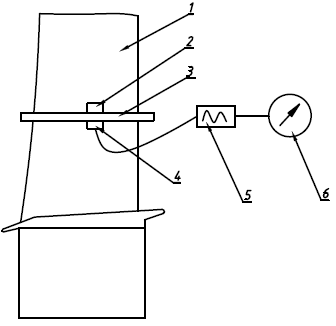
\includegraphics[scale=1]{profile_shape_control}
	\caption{Схема контроля формы профиля лопатки: 1 – лопатка; 2 – светодиод; 3 – шаблон; 4 – фотодиод; 5 –
	аналого-цифровой преобразователь; 6 – индикатор}
	\label{img:profile_shape_control}
\end{figure}

Допуск на  толщину стенки пера, щелей и перемычек $\pm$ 0,3 мм.

Требования назначено из условия обеспечения расчетного режима охлаждения лопатки.

Увеличение толщины стенок лопатки сверх допуска приводит к уменьшению проходного сечения каналов системы охлаждения, что приводит к уменьшению ее эффективности.

Уменьшение толщины стенок лопатки ниже допуска может привести к прогару стенок и выходу лопатки из строя.

Требование для стенок спинки и корыта обеспечивают при окончательной обработке поверхностей спинки и корыта с базированием по замку лопатки. Требование для внутренних стенок обеспечиваются на этапе изготовления заготовки.
Контроль требования осуществляется ультразвуковым толщиномером (рис. ~\ref{img:profile_thk_control}).

\begin{figure}[H]
	\centering
	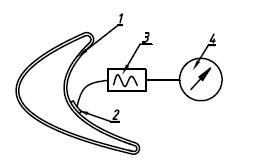
\includegraphics[scale=1]{profile_thk_control}
	\caption{Схема контроля толщины стенок лопатки: 1 – лопатка; 2 – ультразвуковой излучатель/приемник; 3 –
	аналого-цифровой преобразователь; 4 – индикатор}
	\label{img:profile_thk_control}
\end{figure}

Допуск на толщину замка по впадине третьего зуба 0,06 мм.

Требование назначено из условия обеспечения равнопрочности замковой части лопатки и диска.

Уменьшение толщины замка ниже минимального уровня допуска может привести к недопустимому прослаблению материала лопатки и более быстрому ее изнашиванию. Увеличение толщины замка выше максимального уровня допускам может привести к аналогичным результатам применительно к периферийной части диска.

Данное требование обеспечивают при окончательной обработке поверхностей зубьев замкового соединения с базированием по перу, заключенному в кассету из сплава Вуда.

Контроль требования осуществляется микрометром (рис. ~\ref{img:lock_control}).

\begin{figure}[H]
	\centering
	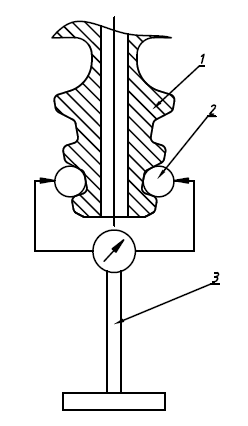
\includegraphics[scale=1]{lock_control}
	\caption{Схема контроля толщины замкового соединения: 1 – замковая часть лопатки; 2 – ролик; 3 – микрометр}
	\label{img:lock_control}
\end{figure}

\subsection{Технологические задачи, возникающие при изготовлении детали}

Основными технологическими задачами, возникающими при изготовлении детали, являются обеспечение качества поверхности профильной части лопатки и обеспечение допусков размеров замковой части лопатки.

К профильной части поверхности лопатки предъявляются высокие требования по обеспечению точности формы профиля и шероховатости поверхности. В связи с этим лезвийная обработка профиля лопатки не допускается. Доводка профиля должно осуществляться только абразивным инструментом.

\subsection{Тип производства и метод работы}

Разработка технологического процесса осуществляется для условий серийного производства. В условиях производства данного типа наиболее целесообразным методом работы является переменно-поточный метод.

Выбор данного метода определяется тем, что использование поточного метода для деталей особой ответственности с множеством контрольных операций затруднительно, а непоточный метод приведет к более низкой загрузке оборудования, удлинит цикл производства и увеличит себестоимость изделия.

\subsection{Технологический анализ конструкции детали}

Конструкция детали состоит из поверхностей сложной пространственной формы, к точности и качеству поверхности которых предъявляются крайне высокие требования.

Перо лопатки образовано трехмерными несимметричными фасонными поверхностями. Также для обеспечения эффективного охлаждения в лопатке выполнена развитая сеть внутренних полостей и 9 рядов отверстий $\diameter$ 0.3 мм на поверхности пера.

Елочный хвостовик лопатки имеет форму призмы с симметричным поперечным сечением сложной формы. В связи со сложной формой профильной части лопатки, при обработке поверхностей хвостовика необходимо использовать специальное приспособление – кассету из сплава Вуда, чтобы обеспечить надежное базирование без риска повредить профильную часть лопатки.

После обработки хвостовик используется в качестве технологической базы для обработки поверхностей пера.

Упрощение геометрических форм лопатки невозможно, так как каждый ее элемент спроектирован для обеспечения эффективного преобразования кинетической энергии потока при соблюдении высоких прочностных свойств конструкции.

Деталь имеет небольшие габариты (40x52x104), что обуславливает сравнительно небольшой объем механической обработки при ее изготовлении. С другой стороны, деталь изготавливается из труднообрабатываемого материала (сплав ЖС36) и является тонкостенной, что не позволяет использовать форсированные режимы обработки.

Вывод: принимая во внимание все вышеперечисленные факторы, стоит признать конструкцию детали нетехнологичной для условий серийного производства. Однако изменение ее конструкции с сохранением эксплуатационных свойств не представляется возможным.

\subsection{Выбор метода изготовления заготовки}
Деталь лопатка в процессе эксплуатации испытывает циклические изгибающие, растягивающие и термоциклические нагрузки. Материал: сталь ЖС-3ВИ. Тип производства: серийное.
Результаты анализа представлены в таблице \ref{tab:technology-detail-properties}.

\pagebreak
\begin{longtable}{|p{6cm}|l|l|}
	\caption{Основные признаки, используемые при выборе заготовки} \label{tab:technology-detail-properties}
	\endfirsthead
	\caption*{\tabcapalign Продолжение таблицы~\thetable}\\[-0.45\onelineskip]
	\hline
	\textbf{Признак} & \textbf{Значение} & \textbf{\makecell{Приоритетный \\ ряд заготовок}} \\ \hline
	\endhead
	\hline
	\textbf{Признак} & \textbf{Значение} & \textbf{\makecell{Приоритетный \\ ряд заготовок}} \\ \hline
	Форма детали & Сложная & О, СК, ОД \\ \hline
	Заготовительные свойства материала & & \\ \hline
	Жидкотекучесть & Удовлетворительная & О \\ \hline
	Пластичность & Неудовлетворительная & (ОД, П) \\ \hline
	Свариваемость & Неудовлетворительная & (СК) \\ \hline
	Обрабатываемость резанием & Неудовлетворительная & (ОД, П) \\ \hline
	Ориентированность структуры & Необходима & ОД, О \\ \hline
	Удельная стоимость материала & Высокая & О, ОД, ПМ \\ \hline
	Ответственность детали & Высокая & ОД, П \\ \hline
	Тип производства & Серийное & П, ОД, СК, О \\ \hline
\end{longtable}

О – отливка; ОД – получение обработкой давлением; П – прокат; СК – сварная или комбинированная; ПМ – полученная методами порошковой металлургии; () – исключение; * - любая (равноприоритетность видов).

Из предварительного анализа следует, что единственным возможным вариантом изготовления лопатки является литье. Данный способ позволяет получить заготовку, максимально приближенную по форме к конечной детали, что немаловажно с учетом высокой стоимости сплава ЖС36. Также, литье является одним из немногих способов получения заготовки, при котором можно изготовить развитую сеть внутренних каналов лопатки (того же эффекта можно достигнуть с помощью порошковой металлургии, но данный способ неприемлем из-за требований к ориентированности структуры заготовки).

В связи с этим, выбирается метод получения заготовки – монокристаллическое литье по выплавляемым моделям. В этом случае точность размеров заготовки достигает 10 квалитета, а шероховатость – значения Ra2,5.

\subsection{Выбор баз и составление маршрутного технологического процесса}

Из-за сложной поверхности пера лопатки и риска ее повреждения, базирование по перу во время обработки хвостовика невозможно. В связи с этим, лопатка помещается в специальное приспособление – кассету и заливается сплавом Вуда. На операциях 005 – 065 базирование производится по поверхностям кассеты. Заготовка лишается шести степеней свободы.

На операциях 085 – 100 базирование производится по профильной (5 степеней свободы) и торцевой (одна степень свободы) поверхностям хвостовика с приложением силы закрепления к противоположному торцу хвостовика. Заготовка лишена шести степеней свободы.